\documentclass[11pt]{scrartcl}

\usepackage[top=1.5cm]{geometry}
\usepackage{url}
\usepackage{float}
\usepackage{listings}
\usepackage{xcolor}
\usepackage{graphicx}
\usepackage{caption}
\usepackage{csquotes}
\usepackage{babel}
\usepackage[T1]{fontenc}
\usepackage[utf8]{luainputenc}
\usepackage{hyperref}

\usepackage[
    backend=biber,
    style=numeric,
    sorting=none
]{biblatex}

\addbibresource{references/references.bib}

\setlength{\parindent}{0em}
\setlength{\parskip}{0.5em}

\newcommand{\youranswerhere}{[Your answer goes here \ldots]}
\renewcommand{\thesubsection}{\arabic{subsection}}

\lstdefinestyle{dmrsql}{
  language=SQL,
  basicstyle=\small\ttfamily,
  keywordstyle=\color{magenta!75!black},
  stringstyle=\color{green!50!black},
  showspaces=false,
  showstringspaces=false,
  commentstyle=\color{gray}}

\lstdefinestyle{dmrJava}{
  language=JAVA,
  basicstyle=\small\ttfamily,
  keywordstyle=\color{magenta!75!black},
  stringstyle=\color{green!50!black},
  showspaces=false,
  showstringspaces=false,
  commentstyle=\color{gray}}

\title{
  \textbf{\large Projektaufgabe 2 } \\
  Phase 1 – Legen der Basis (2.5 P) \\
  {\large Datenmanagement jenseits von Relationen}
}

\author{
  Gruppen Nummer 8 \\
  \large Weilert Alexander, 12119653 \\
  \large Jovanovic Dragana, 11850325
}

\begin{document}

\maketitle\thispagestyle{empty}

Dieses Reporting Template dient der Vorbereitung der Abgabe von Phase 1.

\subsection*{Datengenerator für Matrizen mit Sparsity (0.5 Punkte)}

Zeigen Sie den Code der Funktion generate() als Listing oder Screenshot.
Gehen Sie (kurz) auf die wesentlichen Aspekte ein.

Die Funktion generate(int l, double sparsity) erstellt Tabellen mit der Größe l und einem sparsity.
Beim Start werden die Tabllen A und B gelöscht und neu erstellt. 
Die View C wird gelöscht, da sie in der Laufzeit generiert wird.
Danach werden die Funktionen generateMatrixA(int l, double sparsity) und generateMatrixB(int l, double sparsity) aufgerufen, um Arrays für die Matrizen zu erstellen. 
Beide Funktionen vergleichen die sparsity mit Math.random() und fügen an den entsprechenden Stellen der Matrix entweder eine zufällige Ganzzahl zwischen 1 und 11 oder 0 hinzu.
Die Unterschiede zwischen den Funktionen liegen nur im Array-Aufbau. 
Die Matrix wird entweder mit `int[l-1][l] matrix' oder `int[l][l-1] matrix' definiert, ebenfalls wird dies in der Schleifen- bedingung jeweils verkehrt aufgerufen.
Danach werden die generierten Matrizen mit insertMatrix(String tableName, int[][] matrix) in das DBMS eingefügt. 
Die Funktionen ansatz0(int[][] matrixA, int[][] matrixB) und ansatz1() berechnen die Matrixmultiplikation für C auf unterschiedliche Weise, entweder per Algorithmus oder durch eine Selektion auf A und B. 

\begin{lstlisting}[style=dmrJava]
public void generate(int l, double sparsity) {
    try (Statement statement = this.connection.createStatement()) {
        statement.execute("DROP VIEW IF EXISTS C");
        statement.execute("DROP TABLE IF EXISTS A, B");
        // Create Table
        statement.execute("
        CREATE TABLE A (i INT, j INT, val INT, PRIMARY KEY (i, j))");
        statement.execute("
        CREATE TABLE B (i INT, j INT, val INT, PRIMARY KEY (i, j))");

        int[][] matrixA = generateMatrixA(l, sparsity);
        int[][] matrixB = generateMatrixB(l, sparsity);
        insertMatrix("A", matrixA);
        insertMatrix("B", matrixB);

        ansatz0(matrixA, matrixB); // Matrix Calculator per Algorithm
        ansatz1();                 // Matrix Calculator per Select

    } catch (SQLException e) {
        throw new RuntimeException(e);
    }
}

public int[][] generateMatrixA(int l, double sparsity) {
    Random random = new Random();
    int[][] matrixA = new int[l-1][l];
    System.out.println("--- Matrix A ---");
    for (int i = 0; i < ( l - 1 ); i++) {
        for (int j = 0; j < l; j++) {
            if (random.nextDouble() > sparsity) {
                matrixA[i][j] = random.nextInt(1, 11); 
                // Random value between 0 and 10
            } else {
                matrixA[i][j] = 0;
            }
            System.out.print(matrixA[i][j] + " ");
        }
        System.out.println();
    }
    return matrixA;
}

public int[][] generateMatrixB(int l, double sparsity) {
    Random random = new Random();
    int[][] matrixB = new int[l][l-1];
    System.out.println("--- Matrix B ---");
    for (int i = 0; i < l; i++) {
        for (int j = 0; j < (l - 1); j++) {
            if (random.nextDouble() > sparsity) {
                matrixB[i][j] = random.nextInt(1, 11);
            } else {
                matrixB[i][j] = 0;
            }
            System.out.print(matrixB[i][j] + " ");
        }
        System.out.println();
    }
    return matrixB;
}

public void insertMatrix(String tableName, int[][] matrix) {
    try (Statement statement = this.connection.createStatement())
     {
        StringBuilder insertQuery = new StringBuilder(
            "INSERT INTO " + tableName + " VALUES ");
        for (int i = 0; i < matrix.length; i++) {
            for (int j = 0; j < matrix[i].length; j++) {
                if (matrix[i][j] != 0) {
                    insertQuery.append("(").append(i+1)
                    .append(",").append(j+1).append(",")
                    .append(matrix[i][j]).append("),");
                }
            }
        }
        insertQuery.deleteCharAt(insertQuery.length() - 1);
        statement.executeUpdate(insertQuery.toString());
    } catch (SQLException e) {
        throw new RuntimeException(e);
    }
}
\end{lstlisting}

\subsection*{Import der Matrizen in das DBMS (0.5 Punkte)}

Geben Sie das Create Table Statement für Matrix $A$ an.

\begin{lstlisting}[style=dmrsql]
  CREATE TABLE A (i INT, j INT, val INT, PRIMARY KEY (i, j))
\end{lstlisting}

Für die Übung bereiten Sie eine Demo des Datenimports vor.

Da der Import der Daten für die Matrix automatisch und zufällig passiert, muss mit den Daten gerechnet werden, die generiert werden. 
Mit der folgenden Seite: \href{https://matrixcalc.org/de/}{\textit{Matrix Rechner}}, können Sie sich die Matrixmultiplikation berechnen lassen. 

\subsection*{Wahl des Toy Beispiels (0.5 Punkte)}

Geben Sie Matrix $A$ und $B$ als 2D Array an.
\begin{figure}[H]
    \begin{minipage}[b]{.4\linewidth}
        \begin{center}
            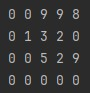
\includegraphics{2d_table_matrix_a.jpg}
        \end{center}
        \caption{2D Ansicht der Tabelle A}
    \end{minipage}
    \hspace{.1\linewidth}
    \begin{minipage}[b]{.4\linewidth}
        \begin{center}
            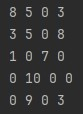
\includegraphics{2d_table_matrix_b.jpg} 
        \end{center}
        \caption{2D Ansicht der Tabelle B}
    \end{minipage}
\end{figure}

Zeigen Sie die äquivalente Darstellung der Matrix $A$ und $B$ in der Datenbank.

\begin{figure}[H]
    \begin{minipage}[b]{.4\linewidth}
        \begin{center}
            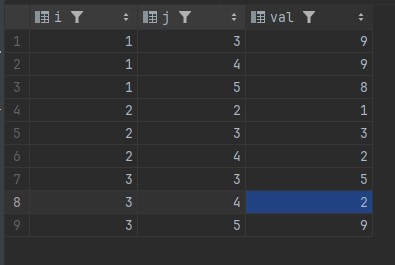
\includegraphics[width=\linewidth]{table_matrix_a.jpg}
        \end{center}
        \caption{Tabelle A im DBMS}
    \end{minipage}
    \hspace{.1\linewidth}
    \begin{minipage}[b]{.4\linewidth}
        \begin{center}
            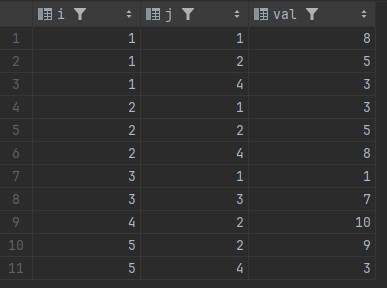
\includegraphics[width=\linewidth]{table_matrix_b.jpg}
        \end{center}
        \caption{Tabelle B im DBMS}
    \end{minipage}
\end{figure}

\subsubsection*{Implementierung von Ansatz 0 (0.5 Punkte)}

Zeigen Sie den Code der Matrixmultiplikation als Listing oder Screenshot.
Erläutern Sie (kurz), welche Laufzeit ihr Algorithmus hat und warum das Kriterium keinen Algorithmus mit sub-kubischer Laufzeit zu wählen erfüllt ist.

\begin{lstlisting}[style=dmrJava]
public void ansatz0(int[][] matrixA, int[][] matrixB) {
    try (Statement statement = this.connection.createStatement())
     {
       statement.execute("DROP TABLE IF EXISTS matrix_algorithm");
       statement.execute("CREATE TABLE 
            matrix_algorithm (i INT, j INT, val INT, PRIMARY KEY (i, j))");
       StringBuilder insertQuery = new StringBuilder(
            "INSERT INTO matrix_algorithm VALUES ");
       int[][] result = new int[matrixA.length][matrixB[0].length];
        System.out.println("--- Matrix Calculator ---");
        for (int i = 0; i < matrixA.length; i++) {
            for (int j = 0; j < matrixB[0].length; j++) {
                for (int k = 0; k < matrixA[0].length; k++) {
                    result[i][j] += matrixA[i][k] * matrixB[k][j];
                }
            insertQuery.append("(").append(i+1).append(",")
            .append(j+1).append(",").append(result[i][j]).append("),");
            System.out.print(result[i][j] + " ");
            }
        System.out.println();
        }
        insertQuery.deleteCharAt(insertQuery.length() - 1);
        statement.executeUpdate(insertQuery.toString());
    } catch (SQLException e) {
        throw new RuntimeException(e);
    }
}
\end{lstlisting}

Ein sub-kubischer Algorithmus bewegt sich in der Laufzeit kleiner O(n$^{3}$).
Unser Algorithmus hat im worst case eine Laufzeit von O(n$^{3}$) und ist somit kubisch. \cite{MatrixMultiplikation},
Ein kubischer Algorithmus muss die Bedingung erfüllen in der Laufzeit O(n$^{3}$) zu sein. \cite{Kubischer},
Dies ist bei uns der Fall, da dieser alle Spalten und Zeilen, der drei verschiedenen for-Schleifen durchläuft, die jeweils die länge n besitzen.

\begin{figure}[H]
    \begin{center}
        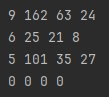
\includegraphics{matrix_algorithm.jpg}
        \caption{Ergebnis C der Matrixmultiplikation anhand des Algorithmus}
    \end{center}
 \end{figure}

\subsubsection*{Implementierung von Ansatz 1 (0.5 Punkte)}
Berechnen Sie von Hand das Ergebnis $C = A \times B$ für ihr Toy Beispiel und geben Sie es nachfolgend an.
 
\begin{figure}
    \begin{center}
        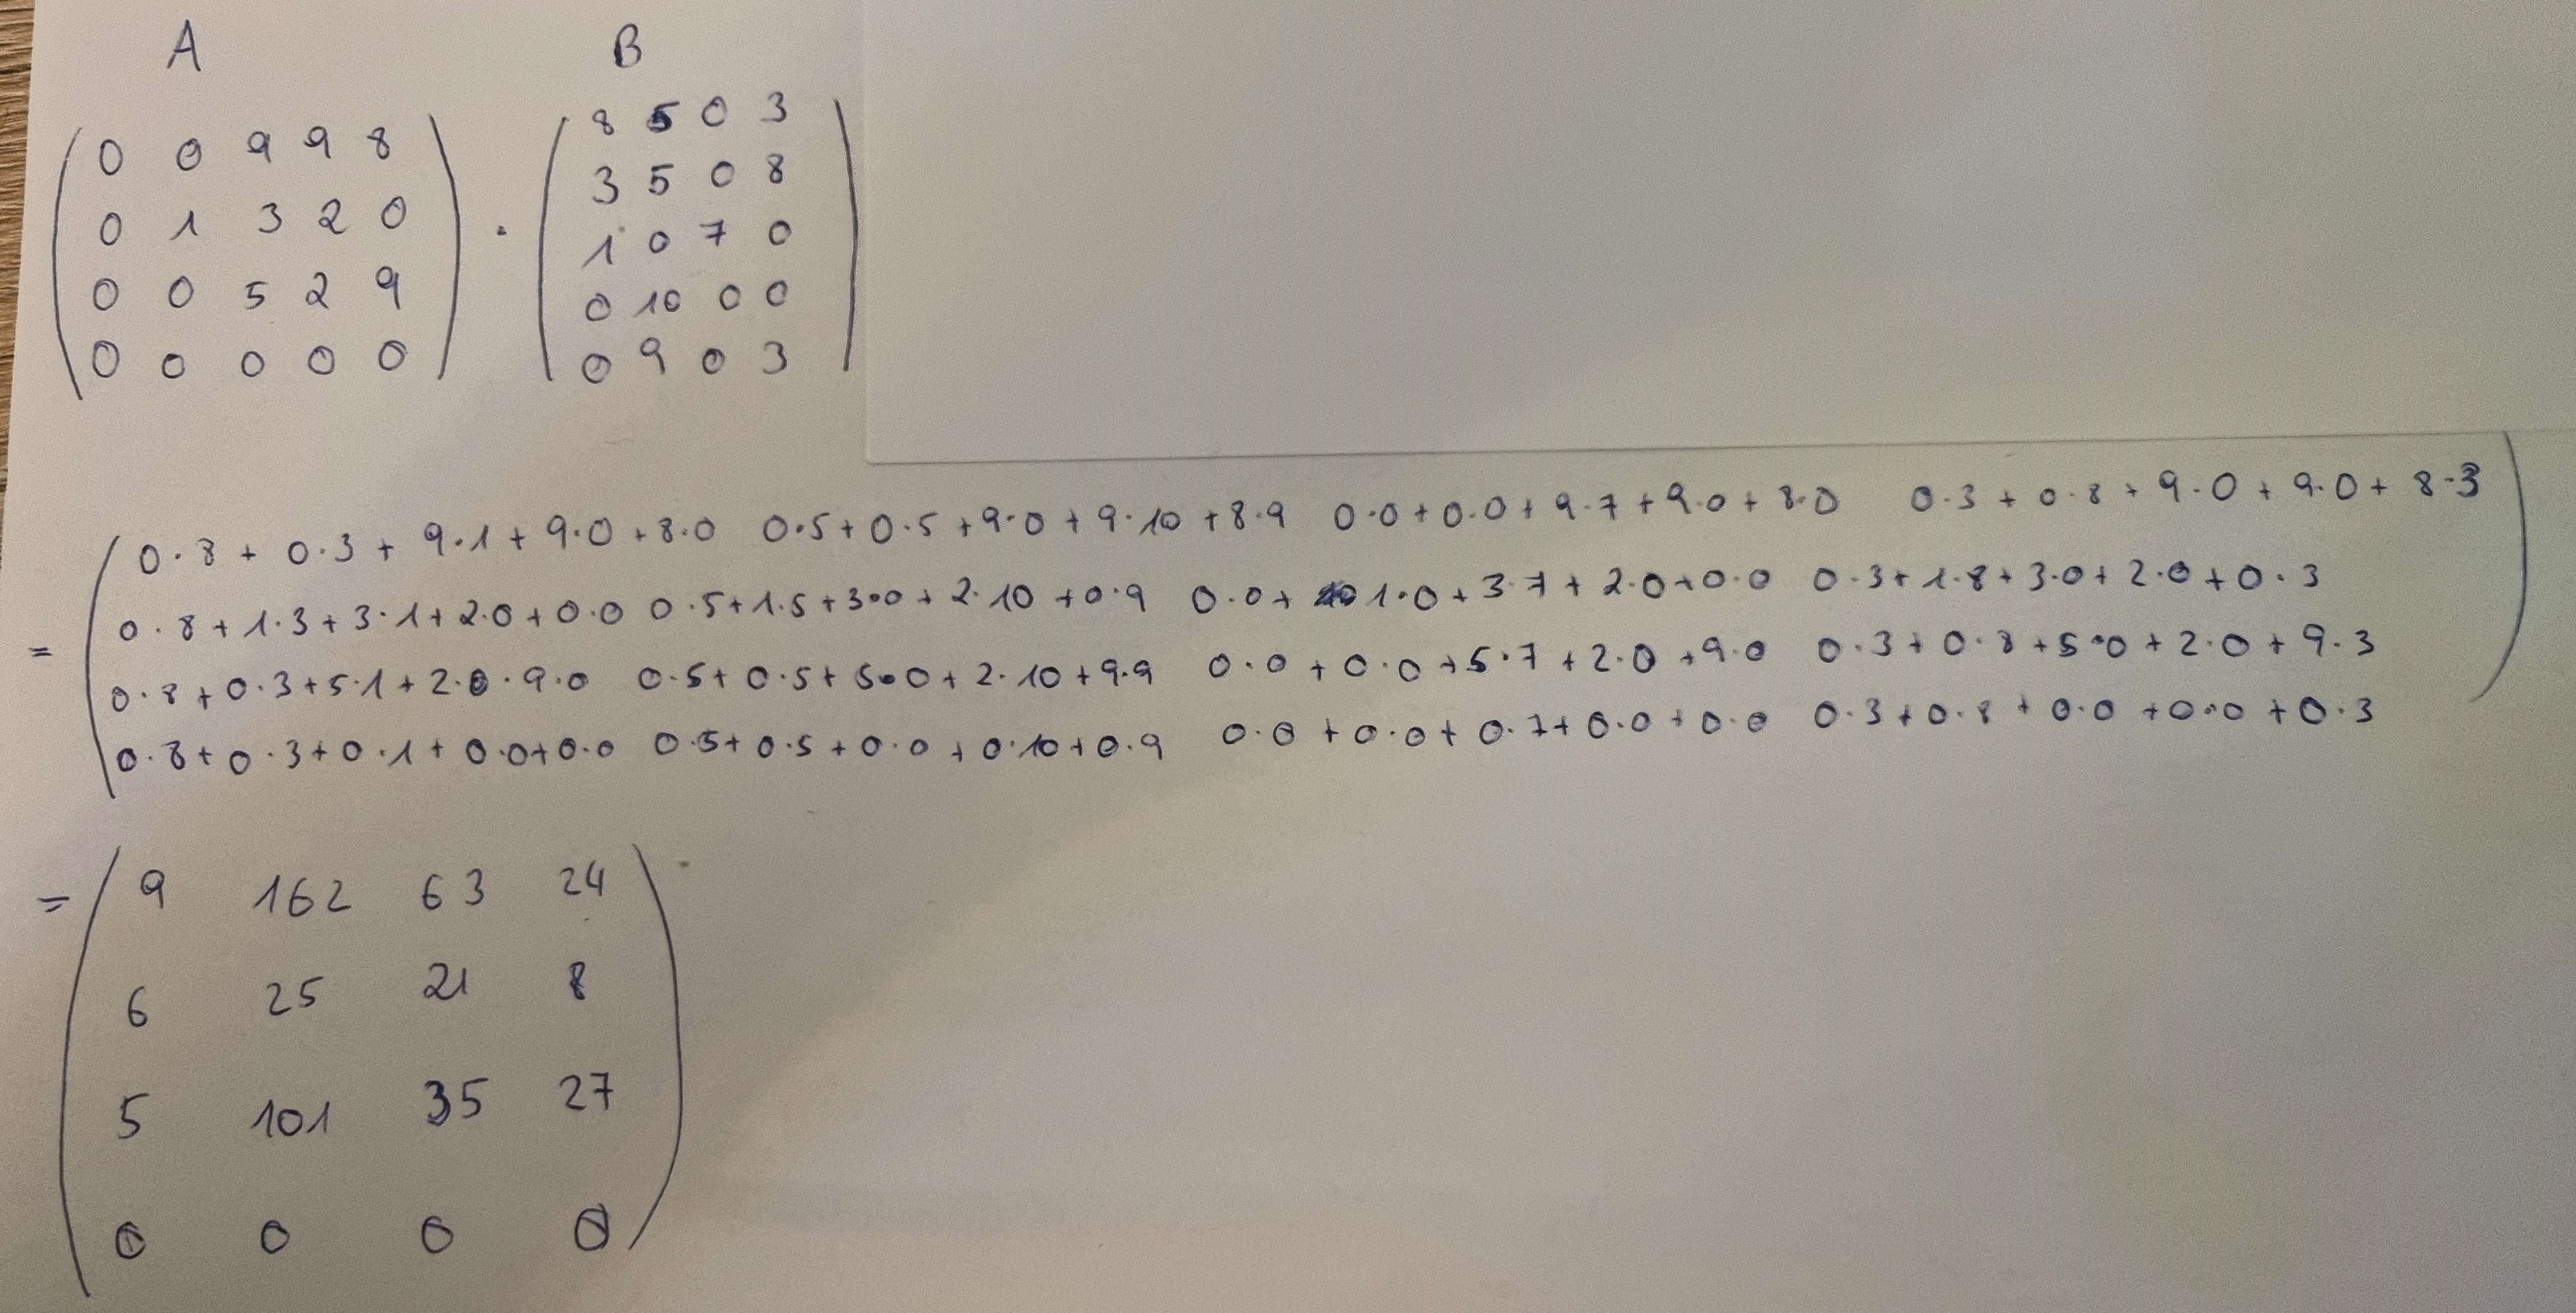
\includegraphics[width=14.5cm,height=8cm]{20240512_200204.jpg}
        \caption{Die von Hand berechnete Matrixmultiplikation}
    \end{center}
 \end{figure}

\begin{lstlisting}[style=dmrJava]
public void ansatz1() {
  try (Statement statement = this.connection.createStatement()) {
      statement.execute("CREATE VIEW C AS " +
          "SELECT a.i, b.j, SUM(A.val * B.val) " +
              "FROM a,  b " +
              "WHERE a.j = b.i " +
              "GROUP BY a.i, b.j");

      } catch (SQLException e) {
      throw new RuntimeException(e);
  }
}
\end{lstlisting}

Zeigen Sie, dass Ihr System $C$ korrekt berechnet (z.B. als Screenshot)

Wir nehmen an, dass das von Hand berechnete Ergebnis richtig bestimmt worden ist.
Vergleichen wir nun das von Hand berechnete, den Ansatz0 und den Ansatz1 so sehen wir eine Übereinstimmung aller Views, weswegen wir nun davon ausgehen können, das der Ansatz1 die Summe richtig berechnet.

\begin{figure}[H]
    \begin{center}
        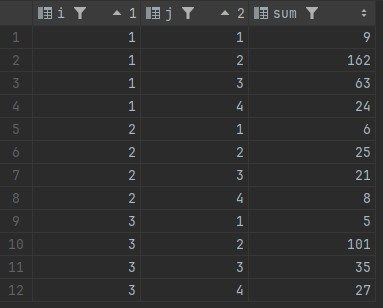
\includegraphics[width=7.5cm,height=5cm]{Selection_View_C.jpg}
        \caption{Vom System Berechnete Matrixmultiplikation über die Selektion aus Ansatz1}
    \end{center}
\end{figure}

\subsection*{Zeitmamagement}

Benötigte Zeit pro Person (nur Phase 1): \\
\textbf{Alexander Weilert: 6h} \\
\textbf{Dragana Jovanovic: 6h}

\subsection*{References}

\begin{table}[H]
  \centering
  \begin{tabular}{c}
    \hline
    \textbf{Important:} Reference your information sources!\tabularnewline
    Remove this section if you use footnotes to reference your information sources.\tabularnewline
    \hline
  \end{tabular}
\end{table}

\printbibliography[title=References]

\end{document}
